\subsubsection{26.12.2015}
\textit{\textbf{Time frame:}} 16:00-22:00

A second pair of shores for the prevention of the entanglement of the cables on the winch coil was installed.

On the ramp for debris there were installed special borders for leading scoring elements to the entrance of the bucket (figure \ref{Gripper2.3}).

\begin{figure}[H]
	\begin{minipage}[h]{1\linewidth}
		\center{\includegraphics[scale=0.2]{3Engineering/5Team_meetings/days_of_meetings/2015.12.26/images/01}}
		\caption{Borders for debris}
		\label{Gripper2.3}
	\end{minipage}
\end{figure}

There used to be a problem that slats, on which the bucket is mounted, bend a lot under it's weight. This day it was found a solution to this problem: it is possible to install a special plate, that will be fixed on the top slat and slide along the surface to which the bottom slat is attached. This plate will rest in the surface and prevent construction from bending.

Today it was created a prototype of this construction (figure \ref{Shiftbuc2.6}, \ref{Shiftbuc2.7}).

\begin{figure}[H]
	\begin{minipage}[h]{0.47\linewidth}
		\center{\includegraphics[scale=0.2]{3Engineering/5Team_meetings/days_of_meetings/2015.12.26/images/02}}
		\caption{Special plate}
		\label{Shiftbuc2.6}
	\end{minipage}
	\hfill
	\begin{minipage}[h]{0.47\linewidth}
		\center{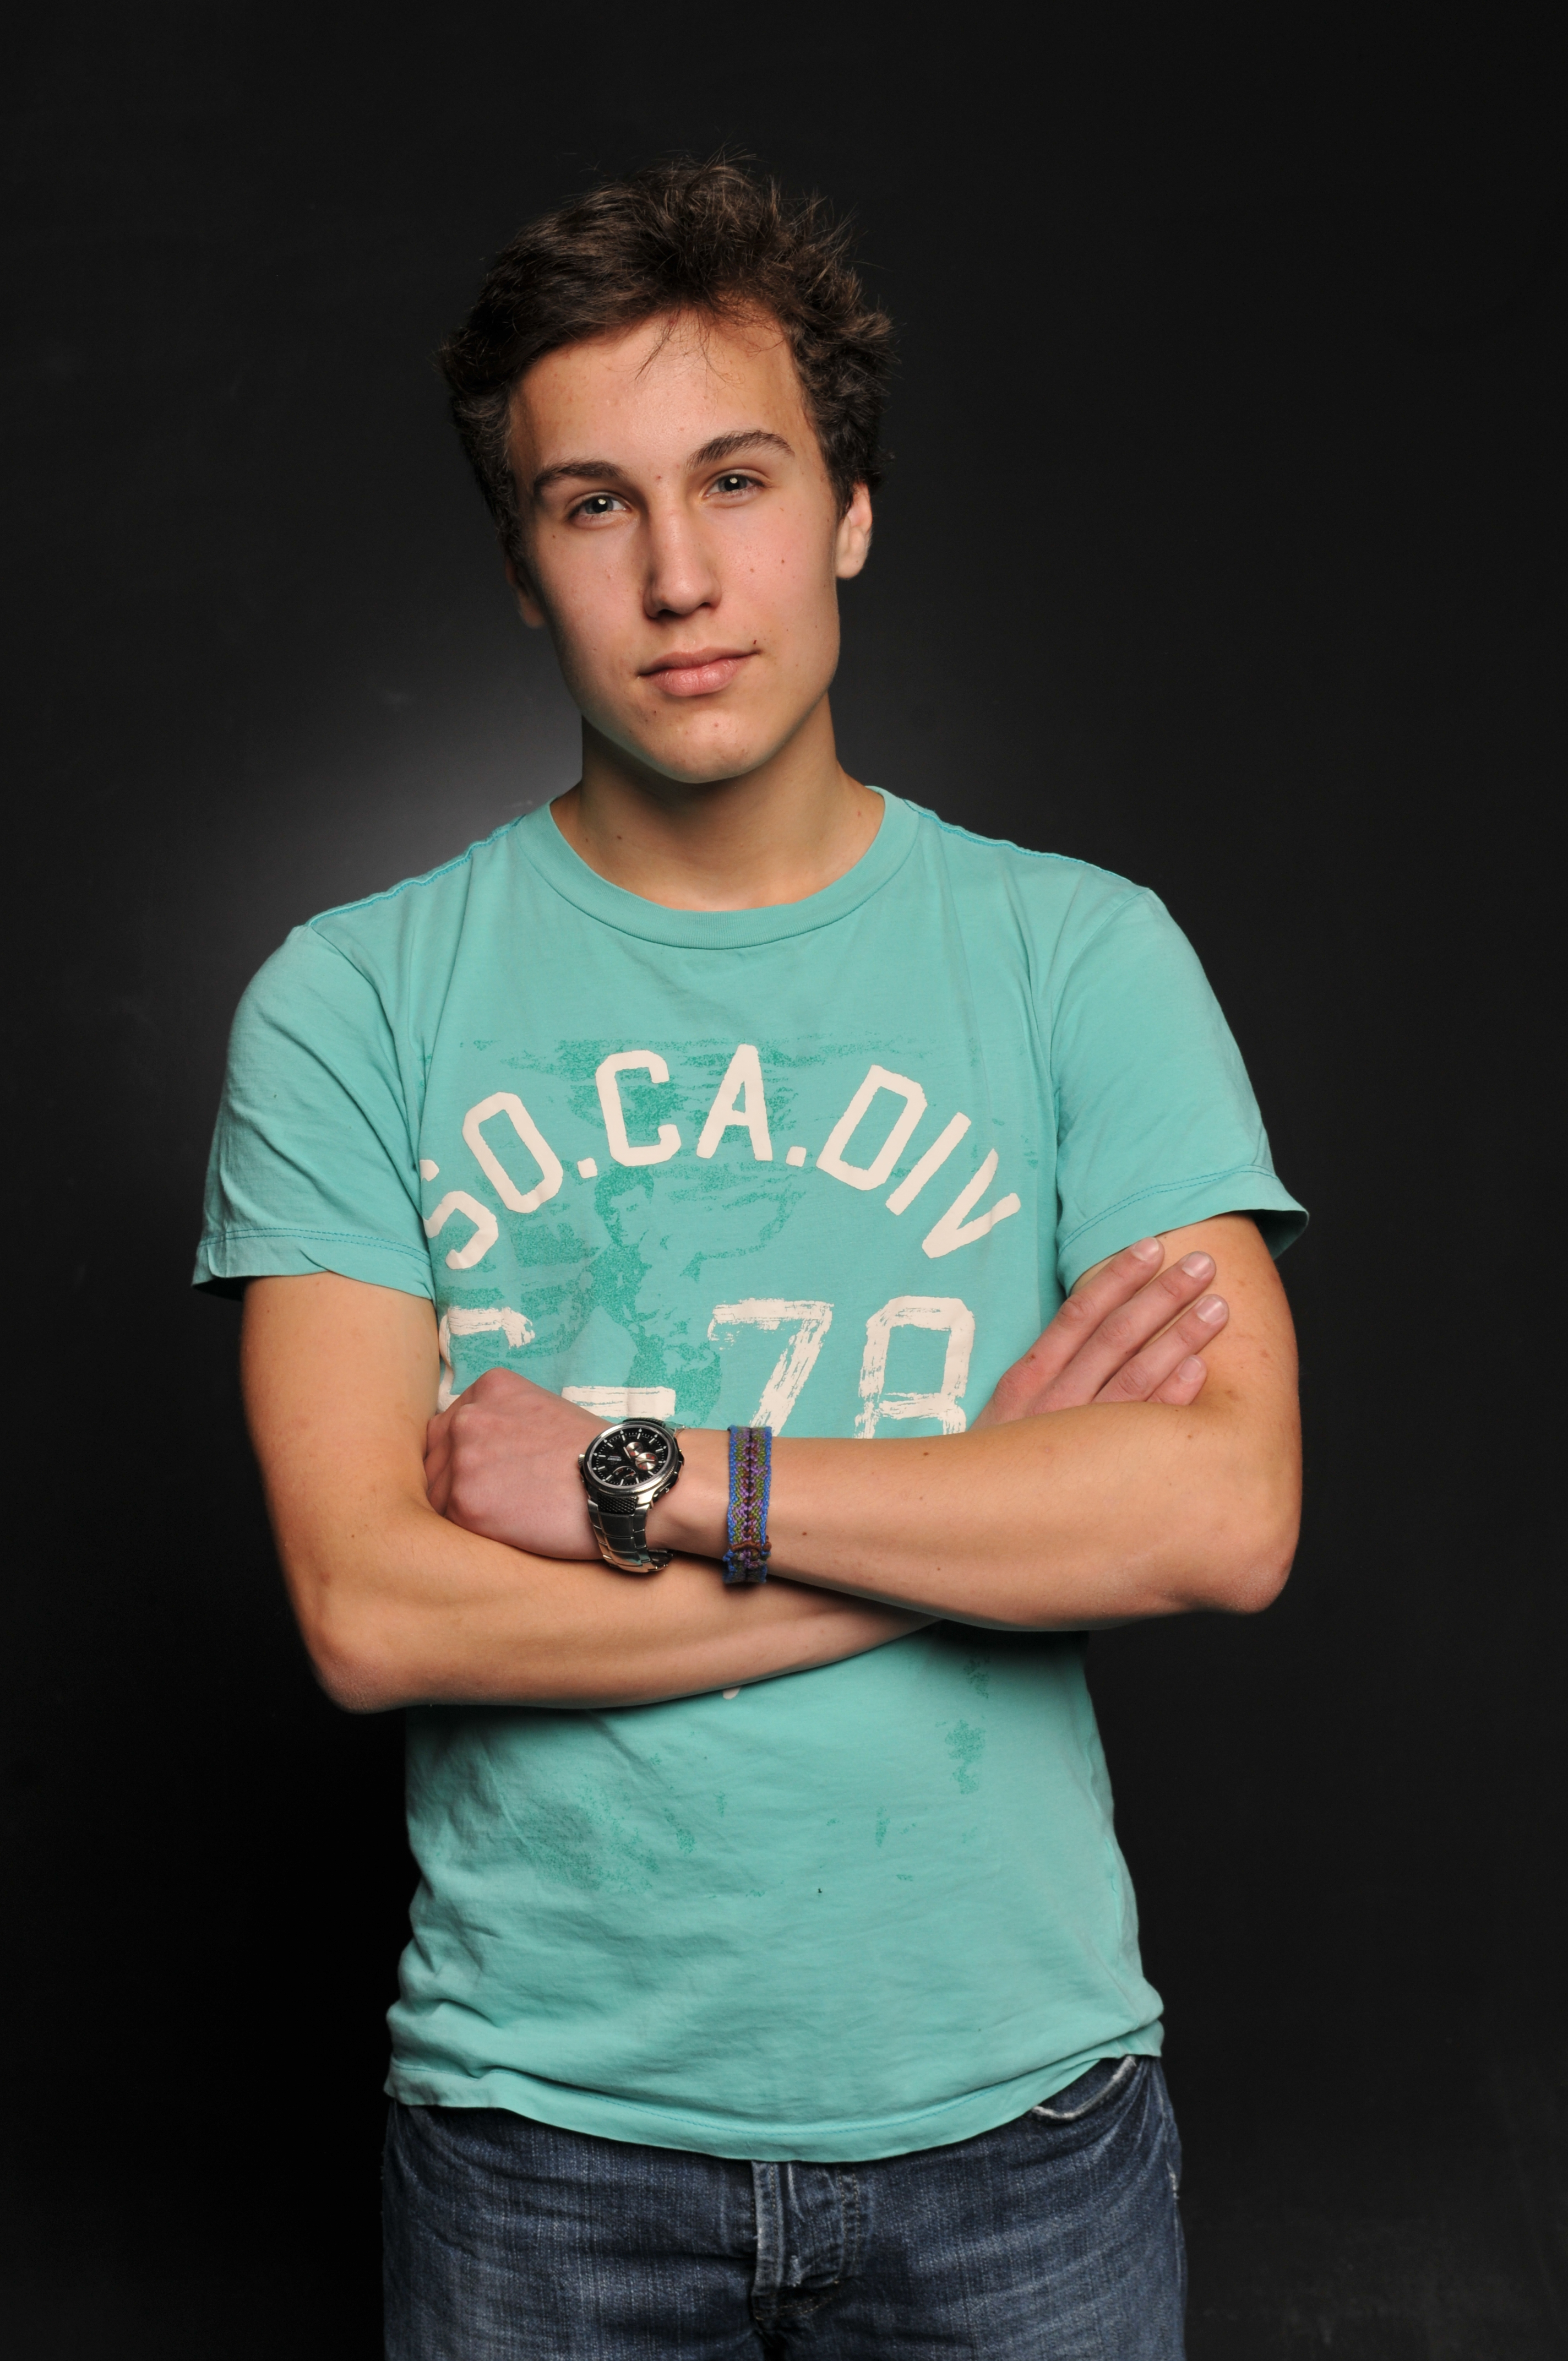
\includegraphics[scale=0.22]{3Engineering/5Team_meetings/days_of_meetings/2015.12.26/images/03}}
		\caption{How does it work}
		\label{Shiftbuc2.7}
	\end{minipage}
\end{figure}
